\section{Assumptions}

This thesis posits that high-level musical concepts manifest over time and remain invariant to specific attributes such as tonal quality, tempo, key, orchestration, signal noise, etc. This is akin to a sheet music composition performed in myriad ways using diverse instruments and styles while preserving its essence.

Abstract features, such as melody, harmony, rhythm, tempo, form, and expression, can be identified irrespective of waveform or production style. This approach offers objective and comprehensive insight into a piece's musical content and meaning, analogous to how analyzing sheet music unveils a composition's underlying structure and intent.

Although a waveform might have limited sheet music representations that accurately encapsulate its musical components, a single sheet music composition can be performed infinitely using various instruments, voices, tempos, and interpretations. The distinct tonal quality of a waveform is significantly influenced by the specific instrument or production technology employed in its creation, complicating the transcription of its sonic properties into precise sheet music notation.

Moreover, this distinct tonal quality is represented by high-level natural language concepts embedded within a rich cultural and sociological tradition.

\begin{figure}[h]
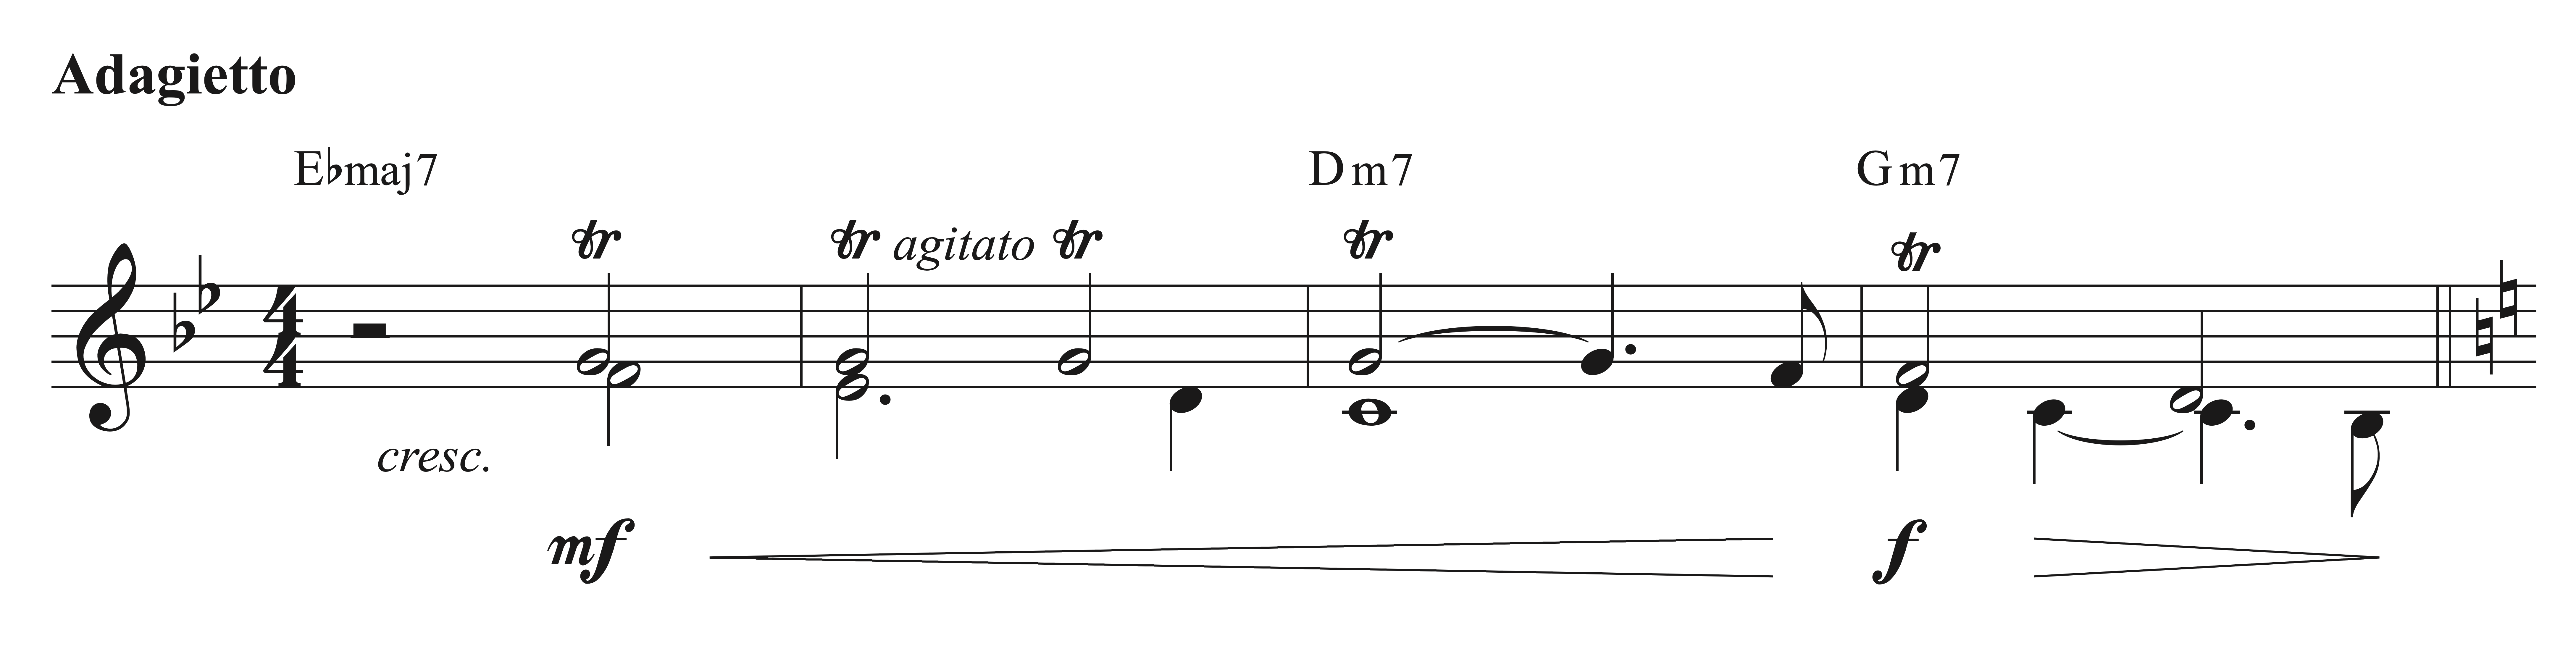
\includegraphics[clip,width=\columnwidth]{figures/images/sheet1.png}% 
\caption{\small{XXXX}}
\label{fig: Sheet music aug 1}
\end{figure}

\begin{figure}[h]
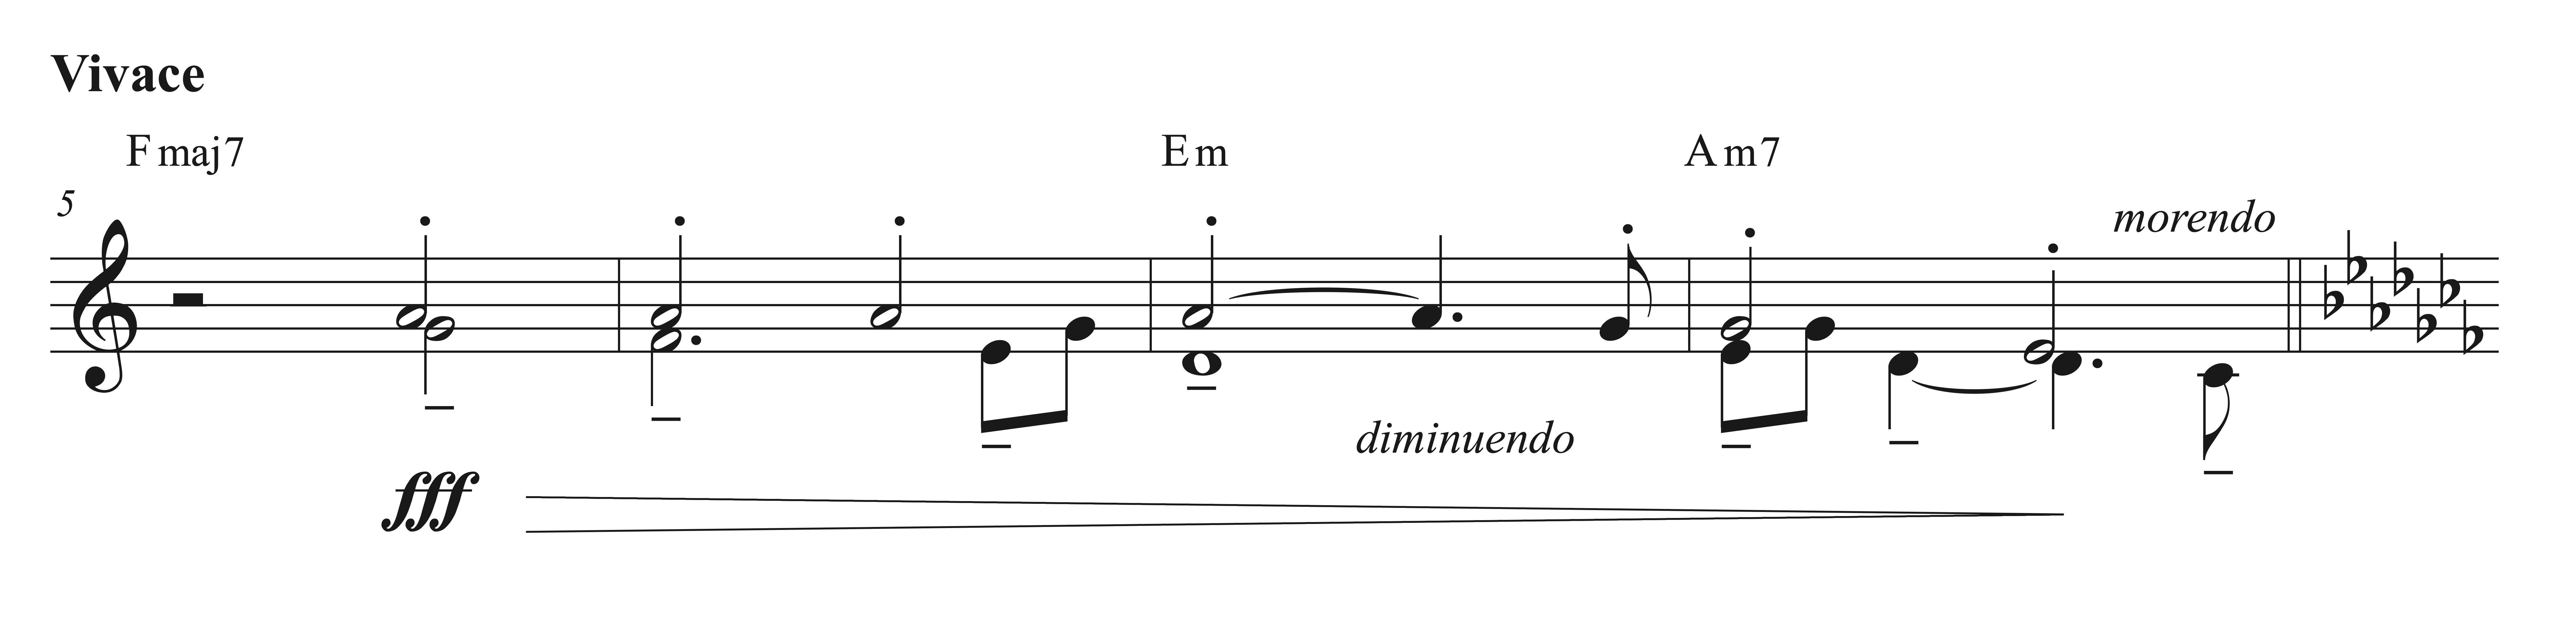
\includegraphics[clip,width=\columnwidth]{figures/images/sheet2.png}% 
\caption{\small{XXXX}}
\label{fig: Sheet music aug 2}
\end{figure}

\begin{figure}[h]
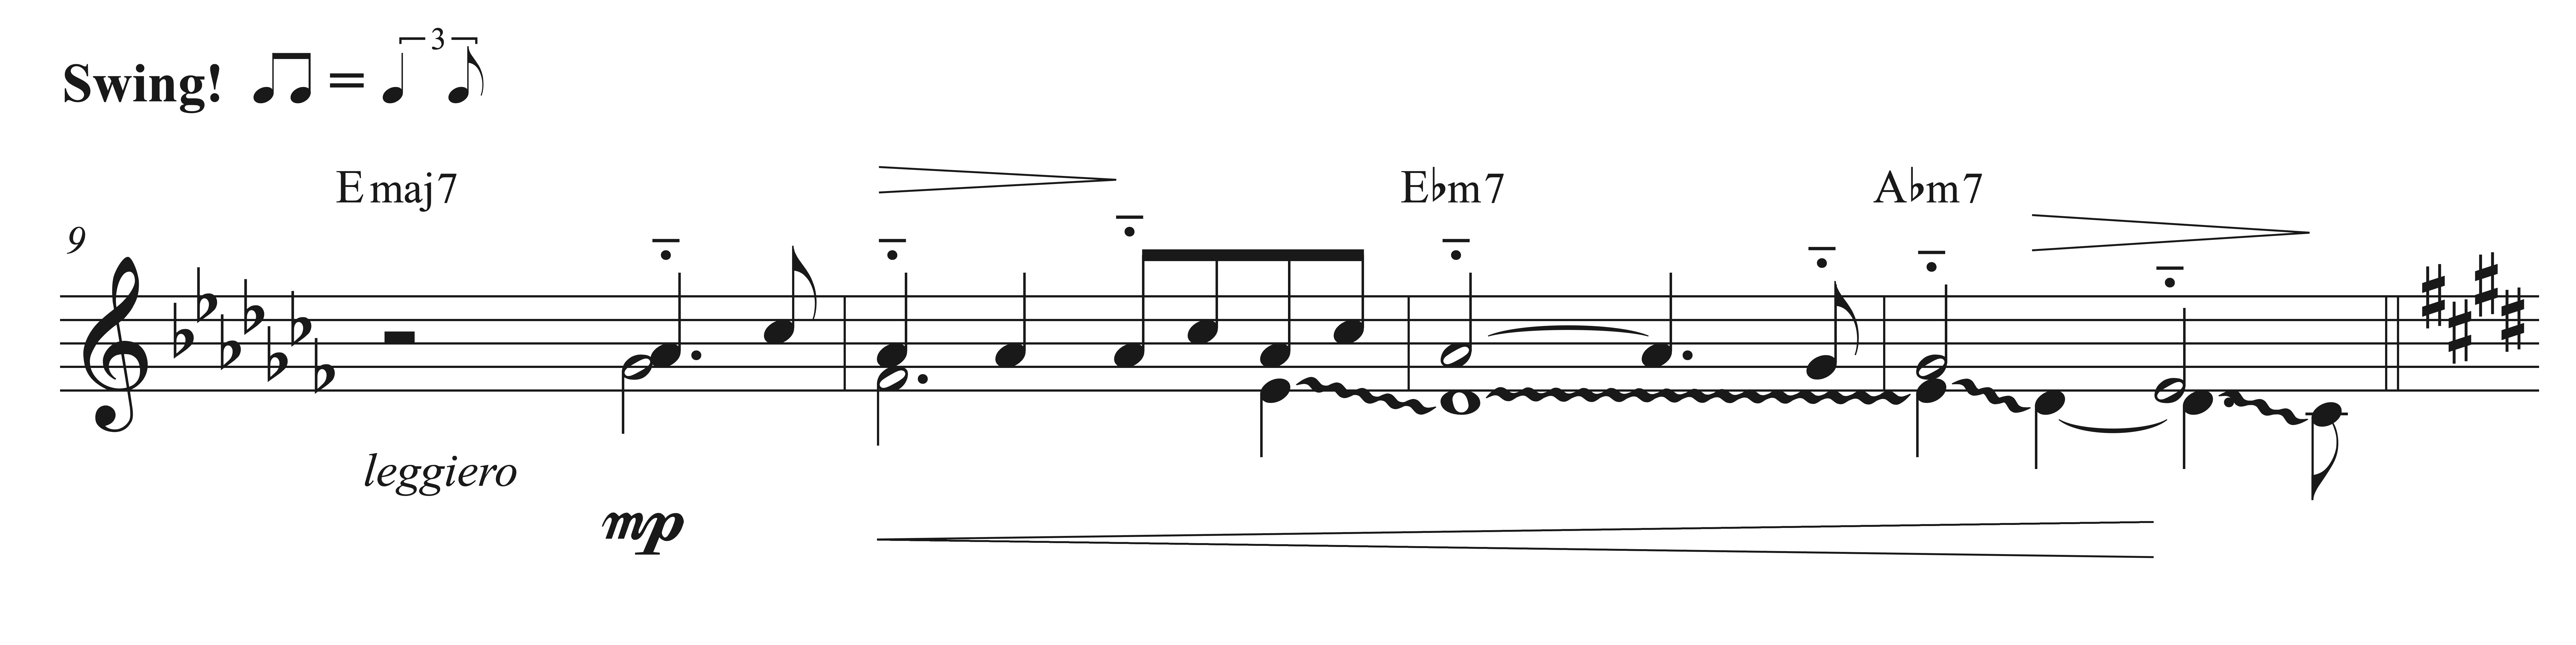
\includegraphics[clip,width=\columnwidth]{figures/images/sheet3.png}% 
\caption{\small{XXXX}}
\label{fig: Sheet music aug 3}
\end{figure}

\begin{figure}[h]
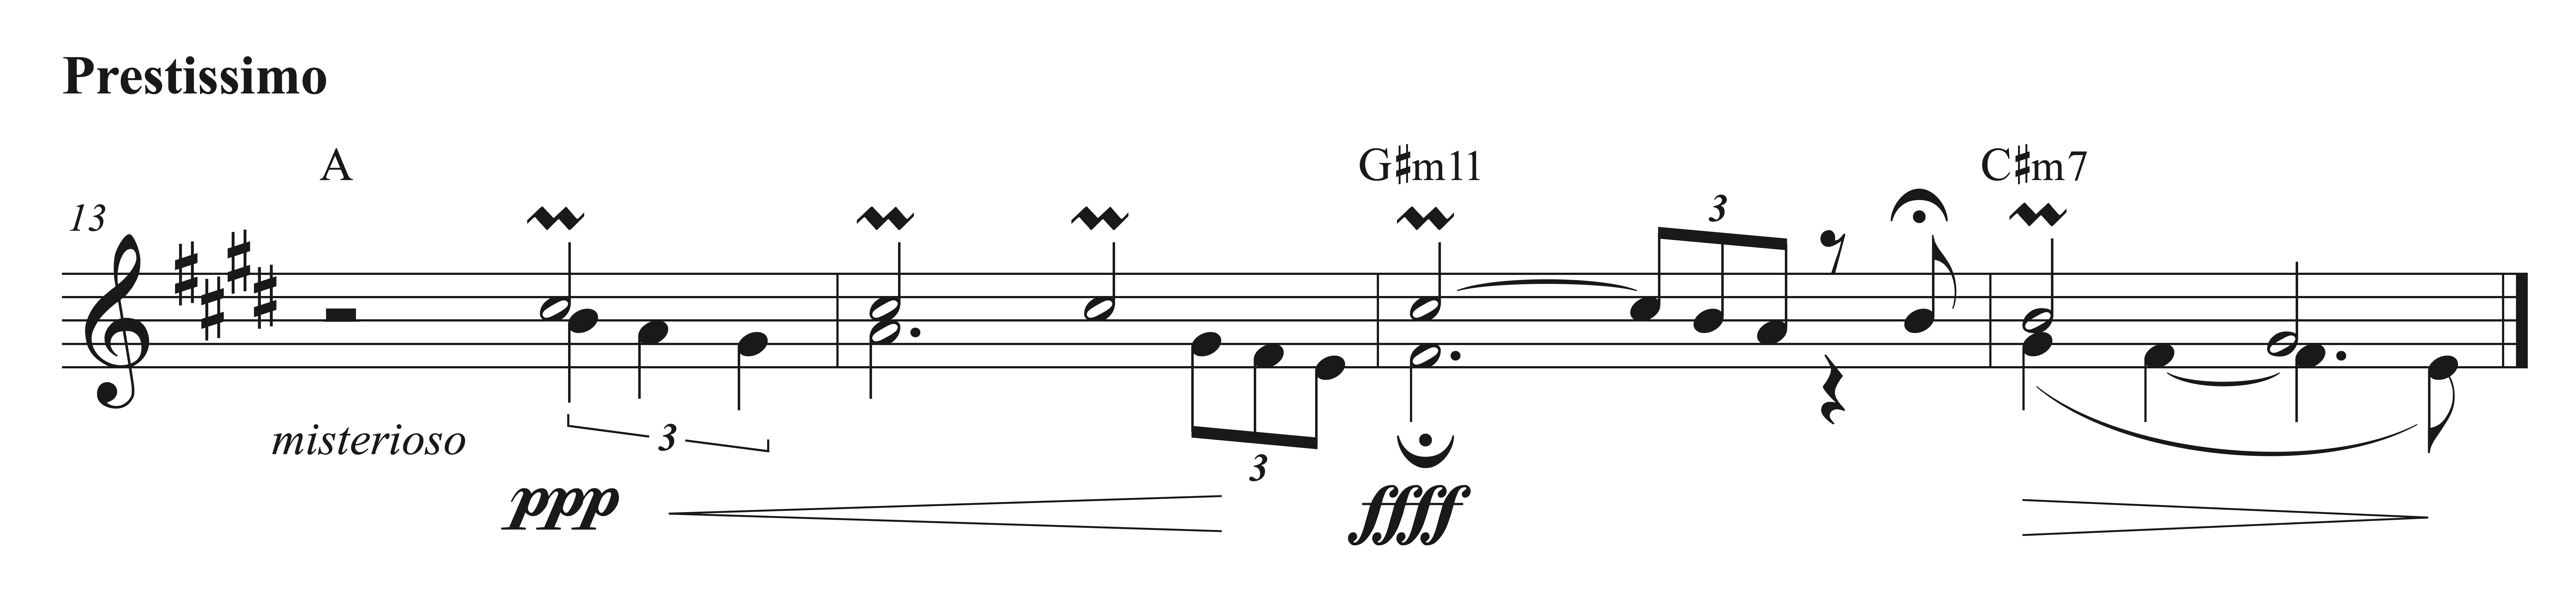
\includegraphics[clip,width=\columnwidth]{figures/images/sheet4.png}% 
\caption{\small{XXXX}}
\label{fig: Sheet music aug 4}
\end{figure}